\chapter{IMPORTANCE OF SEDIMENT GRAIN SIZE TO STOCKS AND STABILITY OF ORGANIC CARBON BURIED IN SEAGRASS SOILS}		\label{another chapter}


\section{Abstract}
Seagrass ecosystems are being considered for conservation and management projects aimed at climate change mitigation based on the organic carbon (C\textsubscript{org}) that they have historically sequestered. Coastal ecosystems inhabited by seagrasses often have more soil C\textsubscript{org} stored than nearby bare sites, but the environmental and ecological factors that control the quantity and stability of seagrass soil carbon are complex and site specific. Here we measured soil carbon density and organic matter (OM) breakdown rates using a standard substrate deployed both buried and on the soil surface, as well as potential environmental and biological drivers of their variation at 45 seagrass-inhabited sites across the South Florida seascape. Total seagrass abundance was positively correlated with soil C\textsubscript{org} density, though variance in data was better explained by sediment characteristics (sediment type, dry bulk density, and sediment grain size). The standard substrate was deployed for six months, with an average exponential breakdown rate, \textit{k}, of 0.33 ± 0.02 yr\textsuperscript{-1} across all samples. Burial only increased OM preservation at sites with muddy, fine sediments where breakdown rates of buried OM were reduced by an average of 22 - 39\% compared to surficial breakdown. At sites with coarser sediments, breakdown rates of OM were at least 55\% greater for buried material. Seagrass abundance had limited (if any) explanatory power for C\textsubscript{org} stock or OM breakdown rates across our study sites, suggesting other factors like geomorphological and hydrological setting have primary control of sediment characteristics, and thus C\textsubscript{org} stocks and breakdown rates. We suggest fine sediments limit porewater exchange through sediments, limiting subsurface microbial decomposition and enhancing C\textsubscript{org} preservation. These findings prompt the reconsideration of Blue Carbon site selection and management, highlighting the importance of environmental controls of C stocks that can be independent of seagrass abundance in these ecosystems.

\section{Introduction}

The capability of some coastal ecosystems to sequester CO\textsubscript{2} and store large carbon stocks is drawing increasing attention as a potential means of inexpensive, conservation-based climate change mitigation \citep{Hiraishi:2014uo}. The term "Blue Carbon" is used to describe the vulnerable organic carbon stocks associated with these coastal vegetated ecosystems (seagrass meadows, mangrove forests, and tidal marshes) that could be lost and emitted as CO\textsubscript{2} during habitat destruction or degradation \citep{Mcleod:2011gs}. The term is also tied to those carbon finance policies and frameworks under development to maximize carbon sequestration through the protection and promotion of carbon-rich ecosystems (collectively called "Blue Carbon strategies"; \citealt{Pendleton:2012hz}). The need to quantify Blue Carbon stocks and assess the relative risk of CO\textsubscript{2} emissions from degraded sites is spurring a flood of investigations into the causal connections between manageable ecosystem attributes and stable, long-term carbon sequestration \citep{Howard:2017jz, Macreadie:2017dt}. Discussions have progressed to the prioritization of optimal Blue Carbon sites, 

\begin{table}[t]
  \centering
  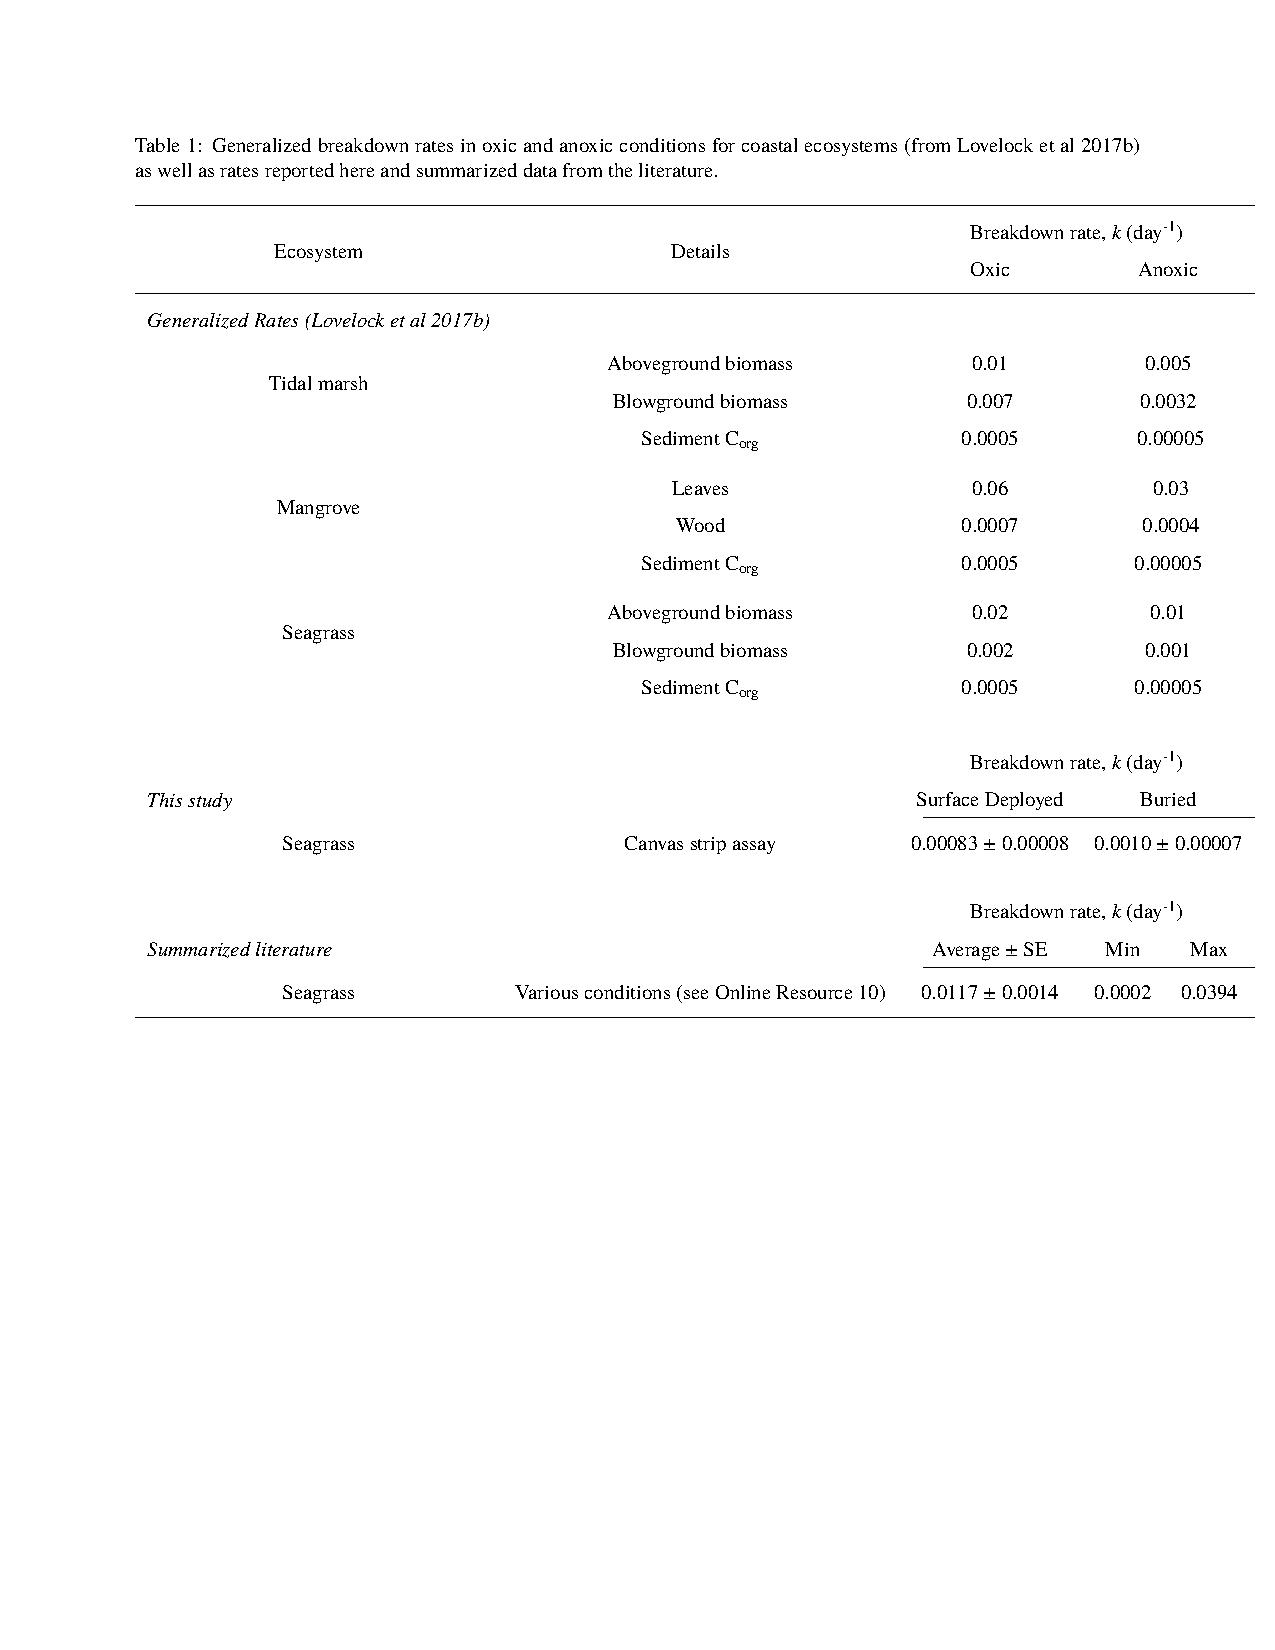
\includegraphics[width=.97\textwidth,clip, trim={2.5cm 10.0cm 0.3cm 3.2cm}]{Figures/chapter2/Tsummary}
\caption[Generalized breakdown rates in oxic and anoxic conditions for coastal ecosystems (from Lovelock et al 2017b) as well as rates reported here and summarized data from the literature.]{Generalized breakdown rates in oxic and anoxic conditions for coastal ecosystems (from Lovelock et al 2017b) as well as rates reported here and summarized data from the literature.}
  \label{table:2T6}
\end{table}

